% beamer presentation
% Karting report

\documentclass{beamer}
% english language
\usepackage[english]{babel}

% tables
\usepackage{tabularx}
\usepackage{graphicx}
\usepackage{hyperref}
\usepackage{listings}
\usepackage{color}

\usetheme{Madrid}

% unibs color #3d5895
% \definecolor{unibs}{RGB}{61,88,149}
\definecolor{unibs}{HTML}{3d5895}


\setbeamercolor{palette primary}{fg=white, bg=unibs}
\setbeamercolor{palette secondary}{fg=white, bg=unibs}
\setbeamercolor{palette tertiary}{fg=white, bg=unibs}
\setbeamercolor{palette quaternary}{fg=white, bg=unibs}

\title{Karting report}
\author{Denis Festa}
\date{\today}

\begin{document}


\begin{frame}
    \titlepage
    \centering
    \includegraphics[width=0.2\linewidth]{unibs-circ-logo.pdf}
\end{frame}

\logo{
\includegraphics[width=0.1\linewidth]{unibs_logo.pdf}}


\section*{User groups}

\begin{frame}
\frametitle{User groups}
\begin{figure}
    \centering
    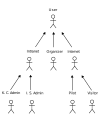
\includegraphics[width=0.4\linewidth]{drawings/users.pdf}
    \caption{User groups}
\end{figure}
\end{frame}

\section*{Use cases}

\subsection*{User}

\begin{frame}
    \frametitle{User}
    \centering
    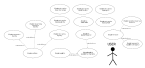
\includegraphics[width=0.9\linewidth]{drawings/uc-user.pdf}
\end{frame}

\subsection*{Intranet}

\begin{frame}
    \frametitle{Kart center administrator}
    \centering
    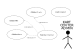
\includegraphics[width=0.9\linewidth]{drawings/uc-kcadmin.pdf}
\end{frame}

\begin{frame}
    \frametitle{Clerk}
    \centering
    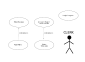
\includegraphics[width=0.9\linewidth]{drawings/uc-clerk.pdf}
\end{frame}

\begin{frame}
    \frametitle{Information system administrator}
    \centering
    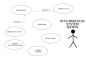
\includegraphics[width=0.9\linewidth]{drawings/uc-isadmin.pdf}
\end{frame}

\subsection*{Extranet}

\begin{frame}
    \frametitle{Organizer}
    \centering
    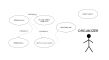
\includegraphics[width=0.9\linewidth]{drawings/uc-organizer.pdf}
\end{frame}

\subsection*{Internet}

\begin{frame}
    \frametitle{Pilot}
    \centering
    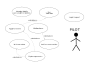
\includegraphics[width=0.9\linewidth]{drawings/uc-pilot.pdf}
\end{frame}

\begin{frame}
    \frametitle{Visitor}
    \centering
    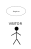
\includegraphics[width=0.3\linewidth]{drawings/uc-visitor.pdf}
\end{frame}

\begin{frame}
\frametitle{Karting center administrator}

\begin{table}
    \tiny
    \begin{tabular}{|p{2cm}|p{6cm}|}
    \hline
    Group name & \textbf{Karting center administrator} \\
    \hline
    Profile data & Name, Surname, e-mail address, password, address, phone number \\
    \hline
    Super group & Intranet \\
    \hline
    Sub group & None \\
    \hline
    Relevant use cases & CRUD on events, races, pilots, tracks, leaderboard, 
    login, logout \\
    \hline
    Read & All \\
    \hline
    Write & All \\
    \hline
    \end{tabular}
    \end{table}

\end{frame}

\begin{frame}
\frametitle{Pilot}

\begin{table}
    \tiny
    \begin{tabular}{|p{2cm}|p{6cm}|}
    \hline
    Group name & \textbf{Pilot} \\
    \hline
    Profile data & Name, Surname, e-mail address, password, address, phone number \\
    \hline
    Super group & Internet \\
    \hline
    Sub group & None \\
    \hline
    Relevant use cases & Create a race, Apply for an event, 
    login, logout \\
    \hline
    Read & All \\
    \hline
    Write & Race, Leaderboard \\
    \hline
    \end{tabular}
    \end{table}

\end{frame}


\section*{Data dictionary}
\begin{frame}
\frametitle{Karting center}

% Table with two columns and 9 rows:
% - Name
% - Synonym
% - Description
% - Example of instance
% - Properties
% - Components
% - Relations
% - Superconcepts
% - Subconcepts

% table 9x2
\begin{table}
\tiny
\begin{tabular}{|p{2cm}|p{6cm}|}
\hline
Name & \textbf{Karting center} \\
\hline
Synonym & Go-karting center \\
\hline
Description & Karting center \\
\hline
Example of instance & 
Name: Mantova Karting Center \newline
\textit{City}: Mantova \newline
\textit{nPilots}: 5937 \newline
\textit{nRaces}: 12485 \newline
\textit{nEvents}:74 \newline
\textit{avgReviewScore}: 3.9 \\
\hline
Properties & 
Name: the name of the karting center\newline
\textit{City}: the city where the karting center is located\newline
\textit{nPilots}: the number of pilots that have raced in the karting center \newline
\textit{nRaces}: the number of races that took place in the karting center \newline
\textit{nEvents}: the number of events that had at least one race hosted by the karting center \newline
\textit{avgReviewScore}: the average score of the reviews of the karting center \\
\hline
Components & None \\
\hline
\end{tabular}
\end{table}

\end{frame}

\begin{frame}
\begin{table}
\tiny
\begin{tabular}{|p{2cm}|p{6cm}|}
\hline
Relations &
KartingCenter\_City (N:1): the city where the karting center is located \newline
KartingCenter\_KartingCenterAdmin (N:1): the karting center administrator of the karting center \newline
KartingCenter\_Clerk (1:N): the clerks of the karting center \newline
KartingCenter\_KartingCenterReview (1:N): the reviews of the karting center \newline
KartingCenter\_Track (1:N): the tracks of the karting center \newline
\textit{KartingCenter\_NPilotsRange} (N:1) the range within the number of pilots that have raced in the karting center falls \newline
\textit{KartingCenter\_NRacesRange} (N:1) the range within the number of races that took place in the karting center falls \newline
\textit{KartingCenter\_NEventsRange} (N:1) the range within the number of events that took place in the karting center falls \newline
\textit{KartingCenter\_KCReviewScoreRange} (N:1) the range within the average score of the reviews of the karting center falls \newline
\textit{KartingCenter\_Event} (N:N) the events the karting center hosted \\
\hline
Superconcepts & None \\
\hline
Subconcepts & None \\
\hline
\end{tabular}
\end{table}
\end{frame}

\begin{frame}
\frametitle{City}
\begin{table}
\tiny
\begin{tabular}{|p{2cm}|p{6cm}|}
\hline
Name & \textbf{City} \\
\hline
Synonym & None \\
\hline
Description & City \\
\hline
Example of instance & 
Name: Mantova \\
\hline
Properties & 
Name: the name of the city \\
\hline
Components & None \\
\hline
Relations &
City\_KartingCenter (1:N): the karting centers located in the city \newline
\textit{City\_Track} (1:N): the tracks (inside a karting center) located in the city \newline
\textit{City\_Event} (N:N): the events that had at least one race on a track of a karting center
located in the city \\
\hline
Superconcepts & None \\
\hline
Subconcepts & None \\
\hline
\end{tabular}
\end{table}
\end{frame}

\begin{frame}
\frametitle{Track}
\begin{table}
\tiny
\begin{tabular}{|p{2cm}|p{6cm}|}
\hline
Name & \textbf{Track} \\
\hline
Synonym & Circuit \\
\hline
Description & Track \\
\hline
Example of instance &
Name: T1 \newline
Length: 700m \newline
\textit{City}: Mantova \newline
\textit{AsphaltType}: resin \newline
\textit{nRentalGoKarts}: 23 \newline
\textit{Difficulty}: Intermediate \newline
\textit{nPilots}: 3873 \newline
\textit{nRaces}: 7437 \newline
\textit{nEvents}: 43 \newline
\textit{avgReviewScore}: 4.2 \\
\hline
Properties &
Name: the name of the track \newline
Length: the length of the track \newline
\textit{City}: the city where the karting center the track belongs to is located \newline
\textit{AsphaltType}: the type of asphalt of the track \newline
\textit{nRentalGoKarts}: the number of rental go-karts available in the track \newline
\textit{Difficulty}: the difficulty of the track \newline
\textit{nPilots}: the number of pilots that have raced on the track \newline
\textit{nRaces}: the number of races that took place on the track \newline
\textit{nEvents}: the number of events that had at least one race on the track \newline
\textit{avgReviewScore}: the average score of the reviews of the track \\
\hline
Components & 
Timetable: the timetable of the track \newline
Leaderboard: a leaderboard of the track \\
\hline
\end{tabular}
\end{table}
\end{frame}

\begin{frame}
\begin{table}
\tiny
\begin{tabular}{|p{2cm}|p{6cm}|}
\hline
Relations &
Track\_KartingCenter (N:1): the karting center the track belongs to \newline
Track\_TrackReview (1:N): the reviews of the track \newline
Track\_Timetable (1:1): the timetable of the track \newline
Track\_Leaderboard (1:N): the leaderboards of the track \newline
Track\_Race (1:N): the races that took place on the track \newline
Track\_GoKart (1:N): the go-karts dedicated to the track \newline
Track\_GoKartModel (N:N): the go-kart models allowed on the track \newline
Track\_TrackAshpalt (N:1): the asphalt of the track \newline
Track\_TrackDifficulty (N:1): the difficulty of the track \newline
Track\_Pilot (N:N): the pilots that have the track as one of their favorite \newline
\textit{Track\_City} (N:1): the city where the karting center the track belongs to is located \newline
\textit{Track\_TrackLengthRange} (N:1): the range within the length of the track falls \newline
\textit{Track\_NPilotsRange} (N:1): the range within the number of pilots that have raced on the track falls \newline
\textit{Track\_NRacesRange} (N:1): the range within the number of races that took place on the track falls \newline
\textit{Track\_NEventsRange} (N:1): the range within the number of events that took place on the track falls \newline
\textit{Track\_TrackReviewScoreRange} (N:1): the range within the average score of the reviews of the track falls \\
\hline
Superconcepts & None \\
\hline
Subconcepts & 
Popular track: a track that is recurrent in the list of favorite tracks of pilots \\
\hline
\end{tabular}
\end{table}
\end{frame}

\begin{frame}
\frametitle{Go-kart}
\begin{table}
\tiny
\begin{tabular}{|p{2cm}|p{6cm}|}
\hline
Name & \textbf{Go-kart} \\
\hline
Synonym & Kart \\
\hline
Description & Go-kart \\
\hline
Example of instance &
Name: T1.1 \newline
GoKartModel: Sodi RX7 \\
\hline
Properties &
Name: the name of the go-kart \newline
\textit{GoKartModel}: the model of the go-kart \\
\hline
Components & None \\
\hline
Relations &
GoKart\_Track (N:1): the track the go-kart is dedicated to \newline
GoKart\_GoKartModel (N:1): the model of the go-kart \\
\hline
Superconcepts & None \\
\hline
Subconcepts & None \\
\hline
\end{tabular}
\end{table}
\end{frame}

\begin{frame}
\frametitle{Timetable}
\begin{table}
\tiny
\begin{tabular}{|p{2cm}|p{6cm}|}
\hline
Name & \textbf{Timetable} \\
\hline
Synonym & None \\
\hline
Description & Timetable \\
\hline
Example of instance &
\textit{TrackName}: T1 \\
\hline
Properties &
\textit{TrackName}: the name of the track \\
\hline
Components & None \\
\hline
Relations &
Timetable\_Track (1:1): the track the timetable belongs to \newline
Timetable\_Reservation (1:N): the reservations of the timetable \\
\hline
Superconcepts & None \\
\hline
Subconcepts & None \\
\hline
\end{tabular}
\end{table}
\end{frame}

\begin{frame}
\frametitle{Leaderboard}
\begin{table}
\tiny
\begin{tabular}{|p{2cm}|p{6cm}|}
\hline
Name & \textbf{Leaderboard} \\
\hline
Synonym & Ranking \\
\hline
Description & Leaderboard \\
\hline
Example of instance &
Title: Best of the week \newline
\textit{TrackName}: T1 \\
\hline
Properties &
Title: the title of the leaderboard \newline
\textit{TrackName}: the name of the track \\
\hline
Components & None \\
\hline
Relations &
Leaderboard\_Track (N:1): the track each leaderboard belongs to \newline
\textit{Leaderboard\_LapTime} (1:N): the lap times the leaderboard focuses on \\
\hline
Superconcepts & None \\
\hline
Subconcepts & None \\
\hline
\end{tabular}
\end{table}
\end{frame}

\begin{frame}
\frametitle{Race}
\begin{table}
\tiny
\begin{tabular}{|p{2cm}|p{6cm}|}
\hline
Name & \textbf{Race} \\
\hline
Synonym & None \\
\hline
Description & Race \\
\hline
Example of instance &
ID: 2036 \newline
Date: 2024-02-15 \newline
Start: 15:00 \newline
End: 15:09 \newline
ForEvent: false \newline
\textit{GoKartingCenterName}: Mantova Karting Center \newline
\textit{TrackName}: T1 \newline
\textit{nPartecipants}: 8 \newline
\textit{fastestLapTime}: 00:00:48.595 \\
\hline
Properties &
ID \newline
Date \newline
Start \newline
End \newline
ForEvent: whether the race was created by an organizer for an event or not \newline
\textit{GoKartingCenterName} \newline
\textit{TrackName}: the name of the track that hosts the race \newline
\textit{nPartecipants} \newline
\textit{fastestLapTime} \\
\hline
Components & None \\
\hline
\end{tabular}
\end{table}
\end{frame}

\begin{frame}
\begin{table}
\tiny
\begin{tabular}{|p{2cm}|p{6cm}|}
\hline
Relations & 
Race\_Track (N:1): the track the race has been raced on \newline
Race\_Reservation (1:1): the reservation that has been made for the race \newline
Race\_Pilot (1:N): the pilots that participated in the race \newline
Race\_Pilot (N:1): the pilot who has this race as his/her last race \newline
Race\_LapTime (1:N): every lap-time of every pilot that participated in the race \newline
Race\_Event (N:1): the event the race is part of \\
\hline
Superconcepts & None \\
\hline
Subconcepts & None \\
\hline
\end{tabular}
\end{table}
\end{frame}

\begin{frame}
\frametitle{Reservation}
\begin{table}
\tiny
\begin{tabular}{|p{2cm}|p{6cm}|}
\hline
Name & \textbf{Reservation} \\
\hline
Synonym & Booking \\
\hline
Description & Reservation \\
\hline
Example of instance &
Date: 2024-02-15 \newline
Start: 15:00 \newline
End: 15:09 \newline
\textit{ReservedByPilot}: Denis Festa \newline
\textit{ReservedByOrganizer}: None \newline
\textit{ConfirmedByClerk}: Jessica \\
\hline
Properties &
Date \newline
Start \newline
End \newline
\textit{ReservedByPilot}: the pilot who made the reservation (this property 
is mutually exclusive with \textit{ReservedByOrganizer}) \newline
\textit{ReservedByOrganizer}: the organizer who made the reservation (this property
is mutually exclusive with \textit{ReservedByPilot}) \newline
\textit{ConfirmedByClerk}: the clerk who confirmed the reservation \\
\hline
Components & None \\
\hline
Relations &
Reservation\_Timetable (N:1): the timetable where the reservation is stored \newline
Reservation\_Pilot (N:1): the pilot who made the reservation \newline
Reservation\_Organizer (N:1): the organizer who made the reservation \newline
Reservation\_Clerk (N:1): the clerk who confirmed the reservation \newline
Reservation\_Race (N:1): the race this reservation has been made for \\
\hline
Superconcepts & None \\
\hline
Subconcepts & None \\
\hline
\end{tabular}
\end{table}
\end{frame}

\begin{frame}
\frametitle{Lap-time}
\begin{table}
\tiny
\begin{tabular}{|p{2cm}|p{6cm}|}
\hline
Name & \textbf{Lap-time} \\
\hline
Synonym & Lap \\
\hline
Description & Lap-time \\
\hline
Example of instance &
LapNumber: 7 \newline
LapTime: 00:00:48.595 \\
\hline
Properties &
LapNumber: the \textit{LapNumber}-th lap \newline
LapTime: the time measured for the \textit{LapNumber}-th lap for 
a particular pilot \\
\hline
Components & None \\
\hline
Relations & 
LapTime\_Pilot (N:1): the pilot who made the lap-time \newline
LapTime\_Race (N:1): the race where the lap-time has been made \newline
\textit{LapTime\_Leaderboard} (N:N): the leaderboards where the lap-time is displayed \\
\hline
Superconcepts & None \\
\hline
Subconcepts & None \\
\hline
\end{tabular}
\end{table}
\end{frame}

\begin{frame}
\frametitle{Application}
\begin{table}
\tiny
\begin{tabular}{|p{2cm}|p{6cm}|}
\hline
Name & \textbf{Application} \\
\hline
Synonym & Request \\
\hline
Description & Application \\
\hline
Example of instance &
Confirmed: true \newline
\textit{EventName}: Mantova Karting Cup 2024 \newline
\textit{RequestFromPilot}: Denis Festa \\
\hline
Properties &
Confirmed: whether the application has been confirmed or not (the organizer who
created the event is the
only one who can accept an application) \newline
\textit{EventName}: the name of the event the application has been made for \newline
\textit{RequestFromPilot}: the pilot who made the application \\
\hline
Components & None \\
\hline
Relations &
Application\_Pilot (N:1): the pilot who made the application \newline
Application\_Event (N:1): the event the application has been made for \\
\hline
Superconcepts & None \\
\hline
Subconcepts & None \\
\hline
\end{tabular}
\end{table}
\end{frame}

\begin{frame}
\frametitle{Event}
\begin{table}
\tiny
\begin{tabular}{|p{2cm}|p{6cm}|}
\hline
Name & Event \\
\hline
Synonym & Tournament \\
\hline
Description & Event \\
\hline
Example of instance &
Name: Mantova Karting Cup 2024 \newline
Price: 100 \newline
\textit{FirstDate}: 2024-02-15 \newline
\textit{OrganizerName}: WD40 \newline
\textit{EventCategory}: Open \newline
\textit{nPartecipants}: 64 \newline
\textit{nRaces}: 12 \newline
\textit{nReviews}: 23 \newline
\textit{avgReviewScore}: 4.5 \\
\hline
Properties &
Name: the name of the event \newline
Price: the price of the event \newline
\textit{FirstDate}: the date of the first race of the event \newline
\textit{OrganizerName}: the username of the organizer who created the event \newline
\textit{EventCategory}: the category of the event (\textit{open, intermediate, pro})\newline
\textit{nPartecipants}: the number of pilots who applied for the event and whose application was confirmed\newline
\textit{nRaces}: the number of races of the event \newline
\textit{nReviews}: the number of written reviews about the event \newline
\textit{avgReviewScore}: the average score of the reviews about the event \\
\hline
Components & None \\
\hline
\end{tabular}
\end{table}
\end{frame}

\begin{frame}
\begin{table}
\tiny
\begin{tabular}{|p{2cm}|p{6cm}|}
\hline
Relations &
Event\_Organizer (N:1): the organizer who created the event \newline
Event\_Application (1:N): the applications received for the event \newline
Event\_Race (1:N): the races of the event \newline
Event\_EventCategory (N:1): the category of the event \newline
Event\_EventReview (1:N): the reviews about the event \newline
\textit{Event\_EReviewScoreRange} (N:1): the range within the average score of the reviews about the event falls \newline
\textit{Event\_Pilot} (N:N): the pilots who applied for the event and whose application was confirmed \newline
\textit{Event\_PriceRange} (N:1): the range within the price of the event falls \newline
\textit{Event\_City} (N:N): the cities where the races of the event took place \newline
\textit{Event\_Track} (N:N): the tracks that hosted the races of the event \newline
\textit{Event\_KartingCenter} (N:N): the karting centers whose tracks hosted the races of the event \\
\hline
Superconcepts & None \\
\hline
Subconcepts & Controversial event, Popular evenet, Upcoming event \\
\hline
\end{tabular}
\end{table}
\end{frame}










% Quando voglio visitare un nuovo arrivo
% utilizzo non una query ma una derivata
% che calcola la query una volta sola

\end{document}